\documentclass{article}

\usepackage{graphicx}
\usepackage{subfig}
\usepackage[hidelinks]{hyperref}

\begin{document}
    \begin{titlepage}
        \centering
        {\bfseries\LARGE Universidad Rey Juan Carlos\par}
        \vspace{1cm}
        {\scshape\Large Ingenier\'ia de Rob\'otica Software \par}
        \vspace{3cm}
        {\scshape\Huge Rob\'otica aerea \par}
        \vspace{3cm}
        {\itshape\Large Problema 2 Tema 3 \par}
        \vfill
        {\Large Autor: \par}
        {\Large Daniel Alejandro Quinga L\'opez \par}
        \vfill
        {\Large Noviembre 2023 \par}
    \end{titlepage}

    \newpage

    El helicóptero a estudiar es el \href{http://www.enstromhelicopter.com/wp-content/uploads/2012/03/enstrom-280fx-specifications.pdf}{\textbf{Enstrom 280FX}}.
    \begin{figure}[h]
        \centerline{\hspace{0cm}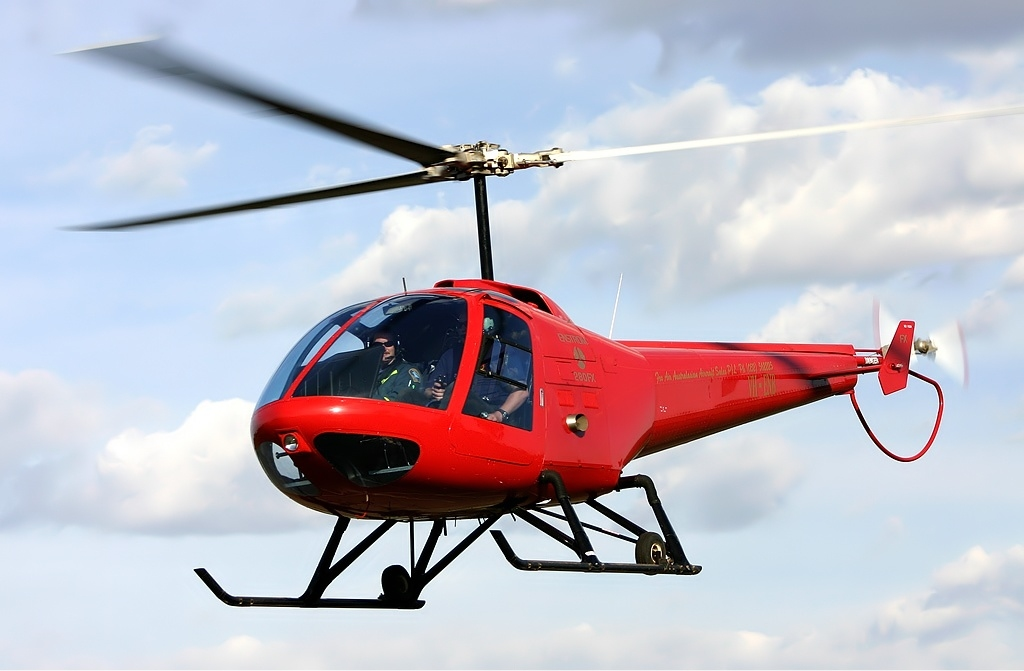
\includegraphics[width=0.66\columnwidth]{Enstrom_280FX_Shark_Geelong_Creek.jpg}}
        \caption{Enstrom 280FX.}\label{fig:figura_1}
    \end{figure}


    Radio del rotor principal: 4,88 metros.
    \newline
    Área del rotor principal: 74,82 $m^2$
    \newline
    Potencia máxima del motor: 167 kW.
    \newline
    Su peso máximo de despegue (MTOW): 1179 kg.
    \newline

    \begin{enumerate}
        \item Velocidad inducida por el rotor principal.
        
        \bigskip
        \begin{center}
            $V_{i} = \sqrt{\frac{W}{2 \rho A}}$.
        \end{center}

        Para un vuelo a punto fijo a 1500m de altitud (condiciones ISA), la velocidad inducida del rotor principal es:
        \begin{center}
            $W = m \cdot g = 1179 \cdot 9.81 = 11566\:N$.
            
            $T = T_{o} - 6,5 \cdot \frac{h}{1000} = 288,15 - 6,5 \cdot \frac{1500}{1000} = 278,4\:K$.

            $p = p_{o}(1 - 0,0065(\frac{h}{T_{o}}))^{5,2561} = 1,013 \cdot 10^5(1 - 0,0065(\frac{1500}{288,15}))^{5,2561} = 84534,5\:Pa$
            
            $\rho = \frac{p}{RT} = \frac{84534,5}{287 \cdot 278,4} = 1,057\:kg/m^3$
            
            $V_{i} = \sqrt{\frac{W}{2 \rho A}} = \sqrt{\frac{11566}{2 \cdot 1,057 \cdot 74.82}} = 8,5513\:m/s$.
        \end{center}
        
        \item Potencia que el motor tiene que proporcionar a los rotores para mantener el vuelo.
        
        \bigskip
        \begin{center}
            $P_{i} = T \cdot V_{i} = \sqrt{\frac{W^3}{2 \rho A}} = 98,904\:kW$.
            \newline
            \newline
            Estimaciones: +10\% rotor de cola, +5\% fuselaje, +10\% resistencia en las palas.
            
            $P_{motor} = P_{i} \cdot 1.25 = 123,63\:kW$.
        \end{center}

        \item Porcentaje de la potencia máxima del motor que esto constituye.
        \begin{center}
            $MaxP_{motor} = 167\:kW \Rightarrow 100\%$

            $P_{motor} = 123,63\:kW \Rightarrow \frac{123,63}{167}\cdot 100 = 74,03\%$.
        \end{center}
        La potencia necesaria en hover es el $74,03\%$ de la máxima.
    
    \end{enumerate}

\end{document}